\titleformat{\section}{\large\bfseries}{}{0pt}{\appendixname\quad\thesection:\quad}

%\setcounter{page}{1}
\setcounter{footnote}{0} %\setcounter{endnote}{0}
\counterwithin{table}{section}
\counterwithin{figure}{section}
\counterwithin{equation}{section}
\renewcommand{\thetable}{\thesection\arabic{table}}
\renewcommand\thefigure{\thesection\arabic{figure}}
\renewcommand{\theequation}{\thesection\arabic{equation}}


\section{CALENDAR OF MONETARY POLICY ANNOUNCEMENTS} \label{sec:calendar}
\sectitlespace

Table \ref{tab:calendar} contains the dates and times of Banxico's monetary policy announcements along with relevant economic data from Mexico and the U.S. released on the same dates.\footnote{ The abbreviations and acronyms used in table \ref{tab:calendar} are as follows: ET is Eastern Time, GDP is gross domestic product, UoM refers to University of Michigan, IGAE is the global economic activity index, IP is industrial production, CPI is the consumer price index, PPI is the producer price index.} Data releases are obtained from Bloomberg. 

Regarding the timing of the announcements, since 2007 the usual one-hour time difference between the capitals of Mexico and the U.S. widens to two hours during some Daylight Saving Time (DST) days. Before 2007, both countries followed the same DST arrangements, from the first Sunday of April to the last Sunday of October.\footnote{ The only exception is 2001, when lawmakers in Mexico shortened the duration of the DST period.} Beginning in 2007, the U.S.---but not Mexico---extended its usage of the DST time, going from the second Sunday of March to the first Sunday of November.

When Banxico announcements occur between the second Sunday of March and the first Sunday of April, and between the last Sunday of October and the first Sunday of November, the relevant Eastern Time (ET) zone times are 11 a.m. (up until 2014) and 3 p.m. (starting in 2015). Seven announcements took place in those weeks prior to 2015 (at 11 a.m. ET) and seven afterwards (at 3 p.m. ET). Those announcements occur more frequently in the Spring than in the Fall because there is a two- to three-week gap in the former and a one-week gap in the latter. In fact, only 2 of the 14 cases fell in October.

In recent years, Banxico's calendar aligns with that of the Fed. On July 1, 2015, Banxico rescheduled the last four monetary policy announcements of that year to one or two business days after the Fed announcements in anticipation to the first increase in the U.S. policy rate since the start of the Great Recession. Since then, Banxico's monetary policy meetings have been scheduled one or two weeks after those of the Fed.

%\documentclass[a4paper,10pt]{article}
\usepackage[labelsep=period,labelfont=bf]{caption}
\usepackage{multirow}
\usepackage{booktabs}
\usepackage{longtable}
\usepackage{pdflscape}
\begin{document}
\begin{tiny}
\begin{center}
\begin{longtable}{p{1.8cm}p{1cm}p{11.7cm}p{1.8cm}p{1cm}p{11.7cm}p{1.8cm}p{1cm}p{11.7cm}}
\caption{Calendar of Monetary Policy Announcements}
\label{tab:calendar}
\endfirsthead
%\multicolumn{3}{c}{\textit{Continued from previous page}} \\
\toprule
 Date & ET & Macroeconomic data from Mexico and the U.S. released on the same day \\
\midrule
\endhead
\bottomrule %\multicolumn{3}{r}{\textit{Continued on next page}} \\
\endfoot
\endlastfoot
\toprule
 Date & ET & Macroeconomic data from Mexico and the U.S. released on the same day \\
\midrule
09-Jan-2004 & 10:00 & MX: Consumer Confidence, IGAE. US: Change in Nonfarm Payrolls, Unemp. Rate. \\
23-Jan-2004 & 10:00 & MX: Trade Balance. \\
06-Feb-2004 & 10:00 & US: Change in Nonfarm Payrolls, Unemp. Rate. \\
20-Feb-2004 & 10:00 & MX: IGAE. US: CPI. \\
12-Mar-2004 & 10:00 & US: UoM Sentiment. \\
26-Mar-2004 & 10:00 & US: UoM Sentiment, Personal Income, Personal Spending. \\
07-Apr-2004 & 10:00 & MX: Gross Fixed Investment. US: Mortgage Applications. \\
23-Apr-2004 & 10:00 & MX: Trade Balance. US: Durable Goods Orders. \\
27-Apr-2004 & 13:15 & US: Consumer Confidence. \\
14-May-2004 & 10:00 & US: CPI, UoM Sentiment, IP. \\
28-May-2004 & 10:00 & US: UoM Sentiment, Personal Income, Personal Spending. \\
11-Jun-2004 & 10:00 & MX: IP. \\
25-Jun-2004 & 10:00 & MX: IGAE. US: GDP, UoM Sentiment. \\
09-Jul-2004 & 10:00 & MX: Trade Balance. \\
23-Jul-2004 & 10:00 & MX: Trade Balance. \\
13-Aug-2004 & 10:00 & US: UoM Sentiment. \\
27-Aug-2004 & 10:00 & US: GDP, UoM Sentiment. \\
10-Sep-2004 & 10:00 &  \\
24-Sep-2004 & 10:00 & MX: IGAE. US: Durable Goods Orders. \\
08-Oct-2004 & 10:00 & US: Change in Nonfarm Payrolls, Unemp. Rate. \\
22-Oct-2004 & 10:00 & MX: Bi-Weekly CPI, Retail Sales. \\
12-Nov-2004 & 10:00 & US: UoM Sentiment, Retail Sales. \\
26-Nov-2004 & 10:00 &  \\
10-Dec-2004 & 10:00 & US: UoM Sentiment. \\
14-Jan-2005 & 10:00 & MX: Gross Fixed Investment. US: IP. \\
28-Jan-2005 & 10:00 & US: GDP. \\
11-Feb-2005 & 10:00 & MX: IP. \\
25-Feb-2005 & 10:00 & US: GDP, Existing Home Sales. \\
11-Mar-2005 & 10:00 &  \\
23-Mar-2005 & 10:00 & MX: Trade Balance. US: CPI, Mortgage Applications, Existing Home Sales. \\
08-Apr-2005 & 10:00 & MX: Gross Fixed Investment. \\
22-Apr-2005 & 10:00 & MX: Bi-Weekly CPI, Trade Balance. \\
13-May-2005 & 10:00 & US: UoM Sentiment. \\
27-May-2005 & 10:00 & MX: Unemployment. US: UoM Sentiment, Personal Income, Personal Spending. \\
10-Jun-2005 & 10:00 &  \\
24-Jun-2005 & 10:00 & MX: Unemployment. US: Durable Goods Orders, New Home Sales. \\
08-Jul-2005 & 10:00 & US: Change in Nonfarm Payrolls, Unemp. Rate. \\
22-Jul-2005 & 10:00 & MX: Bi-Weekly CPI, Trade Balance. \\
12-Aug-2005 & 10:00 & US: UoM Sentiment. \\
26-Aug-2005 & 10:00 & US: UoM Sentiment. \\
09-Sep-2005 & 10:00 & MX: Trade Balance. \\
23-Sep-2005 & 10:00 & MX: Trade Balance. \\
14-Oct-2005 & 10:00 & US: CPI, UoM Sentiment, Retail Sales, IP. \\
28-Oct-2005 & 10:00 & US: GDP, UoM Sentiment. \\
11-Nov-2005 & 10:00 & MX: IP. \\
25-Nov-2005 & 10:00 &  \\
09-Dec-2005 & 10:00 & MX: Trade Balance. US: UoM Sentiment. \\
27-Jan-2006 & 10:00 & US: GDP, New Home Sales. \\
24-Feb-2006 & 10:00 & MX: IGAE, Current Account. US: Durable Goods Orders. \\
24-Mar-2006 & 10:00 & MX: IGAE. US: Durable Goods Orders, New Home Sales. \\
21-Apr-2006 & 10:00 & MX: Retail Sales. \\
26-May-2006 & 10:00 & MX: Retail Sales, Current Account. US: UoM Sentiment, Personal Income, Personal Spending. \\
23-Jun-2006 & 10:00 & MX: Trade Balance. US: Durable Goods Orders. \\
28-Jul-2006 & 10:00 & US: GDP, UoM Sentiment. \\
25-Aug-2006 & 10:00 & MX: IGAE, Current Account. \\
22-Sep-2006 & 10:00 & MX: Bi-Weekly CPI, Retail Sales. \\
27-Oct-2006 & 10:00 & US: GDP, UoM Sentiment. \\
24-Nov-2006 & 10:00 & MX: Retail Sales, Current Account. \\
08-Dec-2006 & 10:00 & MX: Trade Balance. US: Change in Nonfarm Payrolls, UoM Sentiment, Unemp. Rate. \\
26-Jan-2007 & 10:00 & US: Durable Goods Orders, New Home Sales. \\
23-Feb-2007 & 10:00 & MX: Trade Balance, Current Account. \\
23-Mar-2007 & 11:00 & MX: Trade Balance. US: Existing Home Sales. \\
27-Apr-2007 & 10:00 & US: GDP, UoM Sentiment. \\
25-May-2007 & 10:00 & MX: Unemp. Rate, Current Account. US: Existing Home Sales. \\
22-Jun-2007 & 10:00 & MX: Bi-Weekly CPI, Retail Sales. \\
27-Jul-2007 & 10:00 & US: GDP, UoM Sentiment. \\
24-Aug-2007 & 10:00 & MX: Unemp. Rate, Current Account. US: Durable Goods Orders, New Home Sales. \\
21-Sep-2007 & 10:00 & MX: Unemp. Rate. \\
26-Oct-2007 & 10:00 & MX: IGAE. US: UoM Sentiment. \\
23-Nov-2007 & 10:00 & MX: Trade Balance, Current Account. \\
07-Dec-2007 & 10:00 & MX: CPI, Gross Fixed Investment. US: Change in Nonfarm Payrolls, UoM Sentiment, Unemp. Rate. \\
18-Jan-2008 & 10:00 & US: UoM Sentiment. \\
15-Feb-2008 & 10:00 & US: UoM Sentiment, IP. \\
14-Mar-2008 & 11:00 & US: CPI, UoM Sentiment. \\
18-Apr-2008 & 10:00 & MX: Unemp. Rate. \\
16-May-2008 & 10:00 & US: UoM Sentiment, Housing Starts. \\
20-Jun-2008 & 10:00 & MX: Unemp. Rate. \\
18-Jul-2008 & 10:00 & MX: Unemp. Rate. \\
15-Aug-2008 & 10:00 & US: UoM Sentiment, IP. \\
19-Sep-2008 & 10:00 & MX: Unemp. Rate. \\
17-Oct-2008 & 10:00 & MX: IP. US: UoM Sentiment, Housing Starts. \\
28-Nov-2008 & 10:00 &  \\
16-Jan-2009 & 10:00 & MX: IP. US: CPI, UoM Sentiment, IP. \\
20-Feb-2009 & 10:00 & MX: GDP. US: CPI. \\
20-Mar-2009 & 11:00 & MX: Aggregate Supply and Demand. \\
17-Apr-2009 & 10:00 & MX: IP. US: UoM Sentiment. \\
15-May-2009 & 10:00 & US: CPI, UoM Sentiment, IP. \\
19-Jun-2009 & 10:00 & MX: Aggregate Supply and Demand. \\
17-Jul-2009 & 10:00 & MX: IP. US: Housing Starts. \\
21-Aug-2009 & 10:00 & MX: Retail Sales. US: Existing Home Sales. \\
18-Sep-2009 & 10:00 &  \\
16-Oct-2009 & 10:00 & US: UoM Sentiment, IP. \\
27-Nov-2009 & 10:00 &  \\
15-Jan-2010 & 10:00 & US: CPI, UoM Sentiment, IP. \\
19-Feb-2010 & 10:00 & US: CPI. \\
19-Mar-2010 & 11:00 & MX: Aggregate Supply and Demand. \\
16-Apr-2010 & 10:00 & US: UoM Sentiment, Housing Starts. \\
21-May-2010 & 10:00 & MX: Retail Sales. \\
18-Jun-2010 & 10:00 & MX: Retail Sales. \\
16-Jul-2010 & 10:00 & US: CPI, UoM Sentiment. \\
20-Aug-2010 & 10:00 & MX: GDP, IGAE. \\
24-Sep-2010 & 10:00 & US: Durable Goods Orders, New Home Sales. \\
15-Oct-2010 & 10:00 & US: CPI, UoM Sentiment, Retail Sales. \\
26-Nov-2010 & 10:00 &  \\
21-Jan-2011 & 10:00 & MX: Unemp. Rate. \\
04-Mar-2011 & 10:00 & MX: Consumer Confidence. US: Change in Nonfarm Payrolls, Unemp. Rate, Factory Orders. \\
15-Apr-2011 & 10:00 & US: CPI, UoM Sentiment, IP. \\
27-May-2011 & 10:00 & US: UoM Sentiment, Personal Income, Personal Spending. \\
08-Jul-2011 & 10:00 & US: Change in Nonfarm Payrolls, Unemp. Rate. \\
26-Aug-2011 & 10:00 & US: GDP, UoM Sentiment. \\
14-Oct-2011 & 10:00 & US: UoM Sentiment, Retail Sales. \\
02-Dec-2011 & 10:00 & US: Change in Nonfarm Payrolls, Unemp. Rate. \\
20-Jan-2012 & 10:00 & US: Existing Home Sales. \\
16-Mar-2012 & 11:00 & US: CPI, UoM Sentiment, IP. \\
27-Apr-2012 & 10:00 & MX: Trade Balance. US: GDP, UoM Sentiment. \\
08-Jun-2012 & 10:00 & MX: Gross Fixed Investment. \\
20-Jul-2012 & 10:00 & MX: Unemp. Rate. \\
07-Sep-2012 & 10:00 & MX: CPI, Bi-Weekly CPI. US: Change in Nonfarm Payrolls, Unemp. Rate. \\
26-Oct-2012 & 10:00 & US: GDP, UoM Sentiment. \\
30-Nov-2012 & 10:00 & US: Personal Income, Personal Spending. \\
18-Jan-2013 & 10:00 & US: UoM Sentiment. \\
08-Mar-2013 & 10:00 & MX: Gross Fixed Investment. US: Change in Nonfarm Payrolls, Unemp. Rate. \\
26-Apr-2013 & 10:00 & MX: Trade Balance. US: GDP, UoM Sentiment. \\
07-Jun-2013 & 10:00 & MX: CPI, Bi-Weekly CPI. US: Change in Nonfarm Payrolls, Unemp. Rate. \\
12-Jul-2013 & 10:00 & MX: IP. US: UoM Sentiment. \\
06-Sep-2013 & 10:00 & MX: Gross Fixed Investment. US: Change in Nonfarm Payrolls, Unemp. Rate. \\
25-Oct-2013 & 10:00 & MX: Trade Balance. US: UoM Sentiment, Durable Goods Orders. \\
06-Dec-2013 & 10:00 & MX: Gross Fixed Investment. US: Change in Nonfarm Payrolls, UoM Sentiment, Unemp. Rate, Personal Income, Personal Spending. \\
31-Jan-2014 & 10:00 & US: UoM Sentiment, Personal Income, Personal Spending. \\
21-Mar-2014 & 11:00 & MX: Retail Sales. \\
25-Apr-2014 & 10:00 & MX: IGAE. US: UoM Sentiment. \\
06-Jun-2014 & 10:00 & US: Change in Nonfarm Payrolls, Unemp. Rate. \\
11-Jul-2014 & 10:00 & MX: IP. \\
05-Sep-2014 & 10:00 & MX: Consumer Confidence. US: Change in Nonfarm Payrolls, Unemp. Rate. \\
31-Oct-2014 & 11:00 & US: UoM Sentiment, Personal Income, Personal Spending. \\
05-Dec-2014 & 10:00 & MX: Consumer Confidence. US: Change in Nonfarm Payrolls, Unemp. Rate, Factory Orders. \\
29-Jan-2015 & 14:00 & US: Initial Jobless Claims. \\
26-Mar-2015 & 15:00 & US: Initial Jobless Claims. \\
30-Apr-2015 & 14:00 & US: Initial Jobless Claims, Personal Income, Personal Spending. \\
04-Jun-2015 & 14:00 & US: Initial Jobless Claims. \\
30-Jul-2015 & 14:00 & US: Initial Jobless Claims, GDP. \\
21-Sep-2015 & 14:00 & US: Existing Home Sales. \\
29-Oct-2015 & 15:00 & US: Initial Jobless Claims, GDP. \\
17-Dec-2015 & 14:00 & US: Initial Jobless Claims. \\
04-Feb-2016 & 14:00 & MX: Gross Fixed Investment. US: Initial Jobless Claims, Durable Goods Orders, Factory Orders. \\
17-Feb-2016 & 12:17 & (Omitted) \\
18-Mar-2016 & 15:00 & MX: Aggregate Supply and Demand. US: UoM Sentiment. \\
05-May-2016 & 14:00 & US: Initial Jobless Claims. \\
30-Jun-2016 & 14:00 & US: Initial Jobless Claims. \\
11-Aug-2016 & 14:00 & MX: IP. US: Initial Jobless Claims. \\
29-Sep-2016 & 14:00 & US: Initial Jobless Claims, GDP. \\
17-Nov-2016 & 14:00 & US: CPI, Initial Jobless Claims, Housing Starts. \\
15-Dec-2016 & 14:00 & US: CPI, Initial Jobless Claims, Manufacturing PMI. \\
09-Feb-2017 & 14:00 & MX: CPI, Bi-Weekly CPI. US: Initial Jobless Claims. \\
30-Mar-2017 & 15:00 & US: Initial Jobless Claims, GDP. \\
18-May-2017 & 14:00 & US: Initial Jobless Claims. \\
22-Jun-2017 & 14:00 & MX: Bi-Weekly CPI. US: Initial Jobless Claims. \\
10-Aug-2017 & 14:00 & US: Initial Jobless Claims, PPI. \\
28-Sep-2017 & 14:00 & US: Initial Jobless Claims, GDP. \\
09-Nov-2017 & 14:00 & MX: CPI, Bi-Weekly CPI. US: Initial Jobless Claims. \\
14-Dec-2017 & 14:00 & US: Initial Jobless Claims, Retail Sales, Manufacturing PMI. \\
08-Feb-2018 & 14:00 & MX: CPI, Bi-Weekly CPI. US: Initial Jobless Claims. \\
12-Apr-2018 & 14:00 & US: Initial Jobless Claims. \\
17-May-2018 & 14:00 & US: Initial Jobless Claims. \\
21-Jun-2018 & 14:00 & US: Initial Jobless Claims. \\
02-Aug-2018 & 14:00 & US: Initial Jobless Claims, Durable Goods Orders, Factory Orders. \\
04-Oct-2018 & 14:00 & MX: Consumer Confidence. US: Initial Jobless Claims, Durable Goods Orders, Factory Orders. \\
15-Nov-2018 & 14:00 & US: Initial Jobless Claims, Retail Sales. \\
20-Dec-2018 & 14:00 & MX: Retail Sales. US: Initial Jobless Claims. \\
07-Feb-2019 & 14:00 & MX: CPI, Bi-Weekly CPI. US: Initial Jobless Claims. \\
28-Mar-2019 & 15:00 & US: Initial Jobless Claims, GDP. \\
16-May-2019 & 14:00 & US: Initial Jobless Claims, Housing Starts. \\
27-Jun-2019 & 14:00 & MX: Trade Balance. US: Initial Jobless Claims, GDP. \\
15-Aug-2019 & 14:00 & US: Initial Jobless Claims, Retail Sales, IP. \\
26-Sep-2019 & 14:00 & MX: IGAE. US: Initial Jobless Claims, GDP. \\
14-Nov-2019 & 14:00 & US: Initial Jobless Claims, PPI. \\
19-Dec-2019 & 14:00 & US: Initial Jobless Claims, Existing Home Sales. \\
13-Feb-2020 & 14:00 & US: CPI, Initial Jobless Claims, Net Export Sales Corn-Old Crop, Net Export Sales Soybeans-Old, Net Export Sales Wheat-Old, Net Export Sales Cotton-Old. \\
20-Mar-2020 & 15:00 & MX: Aggregate Supply and Demand. US: Existing Home Sales. \\
21-Apr-2020 & 14:00 & MX: International Reserves Weekly. US: Existing Home Sales. \\
14-May-2020 & 14:00 & US: Initial Jobless Claims, Net Export Sales Corn-Old Crop, Net Export Sales Soybeans-Old, Net Export Sales Wheat-Old, Net Export Sales Cotton-Old. \\
25-Jun-2020 & 14:00 & MX: Retail Sales. US: Initial Jobless Claims, Net Export Sales Corn-Old Crop, GDP, Net Export Sales Soybeans-Old, Net Export Sales Wheat-Old, Net Export Sales Cotton-Old, Durable Goods Orders. \\
13-Aug-2020 & 14:00 & US: Initial Jobless Claims, Net Export Sales Corn-Old Crop, Net Export Sales Soybeans-Old, Net Export Sales Wheat-Old, Net Export Sales Cotton-Old. \\
24-Sep-2020 & 14:00 & MX: Bi-Weekly CPI. US: Initial Jobless Claims, Net Export Sales Corn-Old Crop, Net Export Sales Soybeans-Old, Net Export Sales Wheat-Old, Net Export Sales Cotton-Old, New Home Sales. \\
12-Nov-2020 & 14:00 & US: CPI, Initial Jobless Claims, DOE U.S. Crude Oil Inventories, DOE U.S. Gasoline Inventories. \\
17-Dec-2020 & 14:00 & US: Initial Jobless Claims, Net Export Sales Corn-Old Crop, Net Export Sales Soybeans-Old, Net Export Sales Wheat-Old, Net Export Sales Cotton-Old, Housing Starts. \\
11-Feb-2021 & 14:00 & MX: IP. US: Initial Jobless Claims, Net Export Sales Corn-Old Crop, Net Export Sales Soybeans-Old, Net Export Sales Wheat-Old, Net Export Sales Cotton-Old. \\
25-Mar-2021 & 15:00 & MX: Retail Sales, IGAE. US: Initial Jobless Claims, Net Export Sales Corn-Old Crop, GDP, Net Export Sales Soybeans-Old, Net Export Sales Wheat-Old, Net Export Sales Cotton-Old. \\
13-May-2021 & 14:00 & US: Initial Jobless Claims, Net Export Sales Corn-Old Crop, Net Export Sales Soybeans-Old, Net Export Sales Wheat-Old, Net Export Sales Cotton-Old, PPI. \\
24-Jun-2021 & 14:00 & MX: Bi-Weekly CPI, Unemp. Rate. US: Initial Jobless Claims, Net Export Sales Corn-Old Crop, GDP, Net Export Sales Soybeans-Old, Net Export Sales Wheat-Old, Net Export Sales Cotton-Old, Durable Goods Orders. \\
12-Aug-2021 & 14:00 & US: Initial Jobless Claims, Net Export Sales Corn-Old Crop, Net Export Sales Soybeans-Old, Net Export Sales Wheat-Old, Net Export Sales Cotton-Old, WASDE Corn End Stocks, WASDE Soybean Production, PPI, WASDE Corn Yield Per Acre, WASDE Total Wheat End Stocks. \\
30-Sep-2021 & 14:00 & MX: Mexico Copper Production. US: Initial Jobless Claims, Net Export Sales Corn-Old Crop, GDP, Net Export Sales Soybeans-Old, Net Export Sales Wheat-Old, Net Export Sales Cotton-Old, USDA Quarterly Corn Stocks, USDA Quarterly Soybean Stocks. \\
11-Nov-2021 & 14:00 & MX: IP. \\
\bottomrule
\end{longtable}
\end{center}
\end{tiny}
\end{document}

\begin{center}
	[Insert Table \ref{tab:calendar} here.]
\end{center}

\sectitlespace
\section{EXCLUSION OF EXTRAORDINARY MEETINGS} \label{sec:exclusions}
\sectitlespace

Four unscheduled, emergency meetings took place during the sample period. Below are the reasons for excluding them from the analysis. 

\paragraph{April 2004.} On April 23, 2004, Banxico left \textit{el corto} (its monetary policy tool then) unchanged despite recent spikes in inflation, but short-term interest rates declined markedly days after, so Banxico increased it in an unscheduled announcement on April 27. Excluding this meeting, does not influence the few results that use daily data since 2004. 

\paragraph{February 2016.} One week after Banxico's first monetary policy announcement of 2016 (on February 4), the price of oil continued a declining trend and the peso depreciated to a level not seen before (19.2 pesos per dollar), raising concerns about the fiscal position of the Mexican government and the exchange rate pass-through to inflation.
Shortly after noon on February 17, the Finance Secretary and the Governor of Banxico in a joint press conference announced a series of measures to restore confidence to market participants. In addition to a 50-basis-point increase in the policy rate, the measures included fiscal adjustments, which contaminate the response of asset prices to the policy rate decision. 

\paragraph{March and April 2020.} In response to the Covid crisis, Banxico unexpectedly cut its policy rate by 50 basis points on March 20, 2020, six days before a scheduled meeting, and announced four measures to provide liquidity in the foreign exchange and fixed income markets. In another unscheduled meeting on April 21, Banxico announced a reduction in its policy rate of another 50 basis points along with ten measures designed to promote orderly conditions in financial markets and to provide market liquidity.\footnote{The measures included the availability of new dollar auctions (following a Fed announcement of a 60 billion dollar swap line with Banxico on March 19), reductions in reserve requirements for banks and in the cost of the ordinary additional liquidity facility, an expansion of eligible securities and intermediaries for liquidity facilities, and the implementation of new repo facilities. Some measures for market makers to provide liquidity in the sovereign bond market were implemented jointly with the Finance Ministry.} Both extraordinary meetings are excluded from the sample because asset price changes are unlikely to only reflect the reductions in the policy rate, even using intraday windows.\footnote{In unreported regressions that replicate tables \ref{tab:factorid} to \ref{tab:factorfx} but including the two extraordinary meetings of 2020, the estimates of course vary, but the main conclusions in the paper remain.} 

\sectitlespace
\section{\tiie{}-BASED POLICY RATE SURPRISES} \label{sec:tiie}
\sectitlespace

Several considerations need to be taken into account if the \tiie{} were to be used to measure monetary policy surprises. First, it is calculated once a day and thus daily changes are the highest frequency for which \tiie{} can be used, which is relevant given the exchange rate puzzle discussed in section \ref{sec:puzzle}. 

Second, there is a one day difference between the calculation and publication dates, which matters when computing daily changes. The relevant one is the calculation date since it reflects the available information in the market at the time when banks submit their quotes to Banxico for it to calculate the \tiie. Given this timing difference, the data source for the \tiie{} matters. Bloomberg reports the series for the \tiie{} using the calculation date, while Banxico reports the series using the publication date.\footnote{ Daily changes obtained using the publication date do not capture the event of interest (i.e., surprises in monetary policy decisions) since they reflect information one day before the event.}

Third, the timing change of Banxico's monetary policy announcements from 10 a.m. to 2 p.m. ET that started in 2015 matter. The \tiie{} is calculated at 1 p.m. ET with quotes from at least six commercial banks.\footnote{ If less than six banks submit quotes, the calculation time is delayed at most twice in 15-minute intervals. These times increase by one hour in non-overlapping DST days, see section \ref{sec:mptiming}.} This time falls in between the times of the monetary policy announcements preceding and following the timing change. Therefore, the daily changes using the \tiie{} series need to take this into account to ensure that they correctly capture the information before and after each monetary policy announcement. Specifically, prior to 2015, daily changes need to be calculated as the difference in the series the day of the announcement relative to the previous day, but starting in 2015, they need to be obtained as the difference in the series one day after the announcement relative to the day of the announcement.

\tiie{}-based policy rate surprises, however, do not capture the unanticipated part of monetary policy decisions cleanly. First, their correlation with the survey-based (0.67) and swap-based (0.55 with 3-month intraday, 0.63 with 3-month daily, 0.57 with 1-month daily) surprises is not particularly strong. 
Second, \tiie{}-based surprises, when used to estimate equation (\ref{eq:nOneFac}), do not affect the exchange rate nor the 10- and 30-year yields, and weakly affect the 2- and 5-year yields. 

\sectitlespace
\section{THE IMPACT OF MONETARY POLICY ON THE YIELD CURVE} \label{sec:yieldcurve}
\sectitlespace

Table \ref{tab:factorid} shows that a contractionary monetary policy flattens the yield curve. Although this result is in line with the evidence for the U.S. when its policy rate was not constrained by the zero lower bound \parencite{Kuttner:2001, GSS:2005a}, two differences are worth pointing out. First, the magnitude of the yields' response in Mexico is larger than in the U.S. For instance, a 25-basis-point increase in the policy rate raises 2- 5- and 10-year yields by approximately 17, 14 and 11 basis points in Mexico (see table \ref{tab:factorid}) versus 11, 7 and 3 basis points in the U.S. according to the estimates in \textcite{GSS:2005a}. Second, policy rate surprises in Mexico explain a larger fraction of the variability in bond yields (measured by the \(R^2\) statistic) than in the U.S. Specifically, the surprises are the most important factor influencing 2- and 10-year yields in Mexico, with an \(R^2\) of 0.73 and 0.55 versus 0.4 and 0.08 in the U.S., respectively. Keep in mind, however, that the sample periods for the two countries are different, so the figures may not be comparable.

The expectations hypothesis suggests two explanations for the larger influence of policy rate surprises on the yield curve in Mexico compared to the U.S. On the one hand, long-term inflation uncertainty in Mexico may be relatively higher. For instance, surprises in the policy rate can influence long-term inflation compensation in Mexico \parencite[][table 9]{DePooter_etal:2014}, suggesting that inflation expectations are less firmly anchored in Mexico than in the U.S. On the other hand, policy rate surprises may have a larger effect on the term premium. In this case, reach-for-yield investors would rebalance their portfolios in order to take on more or less risk in response to monetary policy decisions, influencing term premia \parencite{HansonStein:2015}. Although an interesting question, quantifying the relative importance of each channel is beyond the scope of this paper.

Table \ref{tab:factordy} shows that the effects of policy rate surprises on the yield curve remain significant when equation (\ref{eq:nOneFac}) is estimated using daily, instead of intraday, data. Moreover, comparing table \ref{tab:factordy} against table \ref{tab:factorid} (over the same sample period) shows that there are gains in the precision of the coefficient estimates and in terms of explanatory power (measured by \(R^2\)) if someone using daily data were to get access to intraday data. The largest gains can be seen at the long end of the curve, where the standard error is half as large and the \(R^2\) doubles when intraday changes are used instead of daily ones. 

Figure \ref{fig:persistprsyc} reports the persistence of the yield curve to policy rate surprises. It shows that Banxico's decisions have persistent effects on the yields of bonds with maturities up to 10 years. In particular, the flattening of the yield curve highlighted in the main text continues in the days following a policy rate tightening. The response of the 2-year yield increases over time,\footnote{Some investors might take time to respond to monetary policy decisions, in which case the sluggish response of the 2-year yield could be attributed to slow-moving capital.} while that of the 10-year yield is relatively more stable.

%\documentclass{article}
\usepackage{graphicx}
\usepackage[margin=1in]{geometry}
\usepackage[outdir=./]{epstopdf}  					% Avoids errors when input figures
\usepackage[labelsep=period,labelfont=bf]{caption}
\usepackage{afterpage}
\input{../Settings/macros_global}			   % Personalized commands
%% Personalized Macros
% Variable Definitions, Equations

%---------------------------------------------------------------
% Variable Definitions
%---------------------------------------------------------------
\providecommand{\tiie}{TIIE28D}
\providecommand{\lastobs}{December 2021}
\providecommand{\lastobsfx}{November 2021}
\providecommand{\lastobsflwbdm}{December 2021}
\providecommand{\lastobsflwtic}{August 2021}
\providecommand{\idxt}{t}
\providecommand{\idxh}{h}
\providecommand{\idxi}{i}
\providecommand{\idxsfwd}{\idxt+\idxh}
\providecommand{\idxslag}{\idxt-1}
\providecommand{\yld}{y}
\providecommand{\ctrls}{z}
\providecommand{\hld}{H}
\providecommand{\depvar}{\Delta \yld_{\idxt}}
\providecommand{\mps}{\Delta x_{\idxt}}
\providecommand{\depvarclean}{\depvar^{*}}
\providecommand{\mpsclean}{\mps^{*}}
\providecommand{\paramB}{\beta}
\providecommand{\intrcpt}{\paramB_{0}}
\providecommand{\slopetrgt}{\paramB_{1}}
\providecommand{\slopepath}{\paramB_{2}}
\providecommand{\assets}{X}
\providecommand{\factors}{F}
\providecommand{\loadings}{\Lambda}
\providecommand{\rotated}{Z}
\providecommand{\rmatrix}{U}
\providecommand{\rtdone}{\rotated_{1}}
\providecommand{\rtdtwo}{\rotated_{2}}
\providecommand{\rtdonereg}{Target_{\idxt}}
\providecommand{\rtdtworeg}{Path_{\idxt}}
\providecommand{\lagidx}{j}
\providecommand{\lagorder}{p}
\providecommand{\lagparam}{\gamma}   %\alpha
\providecommand{\lagoper}{L}
\providecommand{\depvarflw}{\Delta \hld_{\idxt}}
\providecommand{\flows}{w_{\idxt}}
\providecommand{\flowslag}{w_{\idxt - \lagidx}}
\providecommand{\lagsum}{\sum_{\lagidx = 1}^{\lagorder} \lagparam_{\lagidx} \flowslag}
\providecommand{\lagsumh}{\sum_{\lagidx = 1}^{\lagorder} \lagparam^{\lagidx}_\idxh \flowslag}
\providecommand{\dimobs}{T}
\providecommand{\dimassets}{n}
\providecommand{\dimfactors}{k}
\providecommand{\dimnull}{\dimfactors_{0}}
\providecommand{\dimsassets}{\dimobs \times \dimassets}
\providecommand{\dimsfactors}{\dimobs \times \dimfactors}
\providecommand{\dimsloadings}{\dimfactors \times \dimassets}
\providecommand{\errorreg}{\varepsilon_{\idxt}}
\providecommand{\errorfac}{\zeta}
\providecommand{\errorflows}{\nu_{\idxt}}
\providecommand{\Rsqrt}{R^{2}}

\providecommand{\dpv}{y}
\providecommand{\idv}{x}
\providecommand{\omv}{\omega}
\providecommand{\dpvstar}{\dpv^{*}}
\providecommand{\idvstar}{\idv^{*}}
\providecommand{\jobs}{Jobs}
\providecommand{\errortrue}{\varepsilon}
\providecommand{\errormix}{\tau}
\providecommand{\melhs}{\nu}
\providecommand{\merhs}{u}
\providecommand{\mean}{\mu}
\providecommand{\covar}{\sigma}
\providecommand{\corr}{\rho}
\providecommand{\var}{\covar^{2}}
\providecommand{\meanE}{\mean_{\errortrue}}
\providecommand{\meanU}{\mean_{\merhs}}
\providecommand{\meanV}{\mean_{\melhs}}
\providecommand{\varE}{\var_{\errortrue}}
\providecommand{\varU}{\var_{\merhs}}
\providecommand{\varV}{\var_{\melhs}}
\providecommand{\varX}{\var_{\idv}}
\providecommand{\varXstar}{\var_{\idvstar}}
\providecommand{\covarEX}{\covar_{\errortrue \idvstar}}
\providecommand{\covarUE}{\covar_{\merhs \errortrue}}
\providecommand{\covarVE}{\covar_{\melhs \errortrue}}
\providecommand{\covarUX}{\covar_{\merhs \idvstar}}
\providecommand{\covarUY}{\covar_{\merhs \dpvstar}}
\providecommand{\covarVX}{\covar_{\melhs \idvstar}}
\providecommand{\covarVY}{\covar_{\melhs \dpvstar}}
\providecommand{\covarUV}{\covar_{\merhs \melhs}}
\providecommand{\covarWXe}{\covar_{\omv \idv}}
\providecommand{\covarVXe}{\covar_{\melhs \idv}}
\providecommand{\corrUV}{\corr_{\merhs \melhs}}
\providecommand{\corrUX}{\corr_{\merhs \idvstar}}
\providecommand{\corrUY}{\corr_{\merhs \dpvstar}}
\providecommand{\corrVX}{\corr_{\melhs \idvstar}}
\providecommand{\corrVY}{\corr_{\melhs \dpvstar}}
\providecommand{\paramG}{\gamma}
\providecommand{\estimB}{\hat{\paramB}}
\providecommand{\paramSE}{\varE}
\providecommand{\estimSE}{\hat{\paramSE}}
\providecommand{\paramAVB}{s}
\providecommand{\estimAVB}{\hat{\paramAVB}}
\providecommand{\attnfactor}{\lambda}
\providecommand{\plim}{\mathrm{plim}}

\providecommand{\reg}{\delta}
\providecommand{\regVonX}{\reg_{\melhs \idv}}
\providecommand{\regWonX}{\reg_{\omv \idv}}
\providecommand{\regWonXstar}{\reg_{\omv \idvstar}}

%---------------------------------------------------------------
% Equations
%---------------------------------------------------------------
\newcommand{\eqOneFac}{\depvar = \intrcpt + \slopetrgt \mps + \errorreg}
\newcommand{\eqOneFacOV}{\depvar = \intrcpt + \slopetrgt PRS_{\idxt} + \paramB_{2} \Delta VIX_{\idxt} + \paramB_{3} \Delta USY_{\idxt} + \paramB_{4} WTI_{\idxt} + \paramB_{5} \jobs_{\idxt} + \errorreg}
\newcommand{\eqTwoFacP}{\depvar = \intrcpt + \slopetrgt \rtdonereg + \slopepath \rtdtworeg + \errorreg}
\newcommand{\eqTwoFacF}{\depvarflw = \intrcpt + \slopetrgt \rtdonereg + \slopepath \rtdtworeg + \errorreg}
\newcommand{\eqPCA}{\assets = \factors \loadings + \errorfac}
\newcommand{\eqRotation}{\rotated = \factors \, \rmatrix}
\newcommand{\eqFlows}{\flows = \intrcpt + \slopetrgt \rtdonereg + \slopepath \rtdtworeg + \lagsum + \eta^{'} \ctrls_{\idxslag} + \errorflows}
\newcommand{\eqAsym}{\yld_{\idxt} = \intrcpt + \paramB_{1} \rtdonereg \mathds{1} \left(\rtdonereg > 0 \right) + \paramB_{2} \rtdonereg \mathds{1} \left(\rtdonereg < 0 \right) \\ + \paramB_{3} \rtdtworeg \mathds{1} \left(\rtdtworeg > 0 \right) + \paramB_{4} \rtdtworeg \mathds{1} \left(\rtdtworeg < 0 \right) + \errorreg}

\newcommand{\eqDGP}{\dpvstar &= \paramB \idvstar + \errortrue}
\newcommand{\eqDGPme}{\dpv = \paramB \idv + \errormix = \paramB \idv + \eqErrormix}
\newcommand{\eqDGPov}{\dpvstar = \paramB \idvstar + \paramG \omv +  \errortrue}
\newcommand{\eqMEdpv}{\dpv &= \dpvstar + \melhs}
\newcommand{\eqMEidv}{\idv &= \idvstar + \merhs}
\newcommand{\eqAtten}{\attnfactor = \frac{\varXstar}{\varXstar + \varU}}
\newcommand{\eqAttenInLine}{\attnfactor = \varXstar / \left(\varXstar + \varU\right) }
\newcommand{\eqErrormix}{\errortrue - \paramB \merhs + \melhs}

\newcommand{\eqPlimBstd}{\plim \left( \estimB \right) = \frac{cov(\idv, \dpvstar)}{var(\idv)} = \frac{cov(\idvstar + \merhs, \paramB \idvstar + \errortrue)}{var(\idvstar + \merhs)} = \paramB \frac{\varXstar}{\varXstar + \varU} = \paramB \attnfactor}
\newcommand{\eqPlimBstdshort}{\plim (\estimB) = \paramB \attnfactor}

\newcommand{\eqPlimSstd}{\plim \left( \estimAVB \right) = \attnfactor \paramAVB + \attnfactor(1 - \attnfactor) \paramB^{2}}

\newcommand{\eqPlimBnew}{\plim \left( \estimB \right) 
	= \frac{cov(\idv, \dpv)}{var(\idv)} 
	= \frac{cov(\idvstar + \merhs, \paramB \idvstar + \paramG \omv + \errortrue)}{var(\idvstar + \merhs)} 
	= \frac{\paramB \varXstar + \paramG \covarWXe}{\varXstar + \varU}  }

\newcommand{\eqPlimBbias}{\plim \left( \estimB \right)
	= \paramB \frac{\varXstar}{\varX} + \paramG \frac{\covarWXe}{\varX}
	= \paramB \attnfactor + \paramG \regWonX}

\providecommand{\errordepvar}{e_{y}}
\providecommand{\errormps}{e_{x}}
\newcommand{\eqMEdepvar}{\depvar &= \depvarclean + \errordepvar}
\newcommand{\eqMEmps}{\mps &= \mpsclean + \errormps}

\newcommand{\eqLPrhs}{\alpha_{\idxh} + \beta^{1}_{\idxh} \; \rtdonereg +  \beta^{2}_{\idxh} \; \rtdtworeg + \eta^{'}_{\idxh} \ctrls_{\idxslag}  + u_{\idxsfwd}}

\newcommand{\eqLPprices}{\yld_{\idxsfwd} - \yld_{\idxslag} = \eqLPrhs} 

\newcommand{\eqLPflows}{\hld_{\idxsfwd} - \hld_{\idxslag} = \eqLPrhs} 

\newcommand{\eqLP}{\yld_{\idxsfwd} - \yld_{\idxslag} = \alpha_{\idxh} + \gamma_{\idxh} \mps + u_{\idxsfwd}} 			    % Personalized commands

\begin{document}
	\begin{figure}[tbph]
		\caption{Persistence of the Yield Curve Response to Policy Rate Surprises} \label{fig:persistprsyc}
		\begin{center}								% center the minipage on the line
			\begin{minipage}{0.9\linewidth}
				\begin{center}							% center the figure inside the minipage
					\label{fig:persistprsyc}
					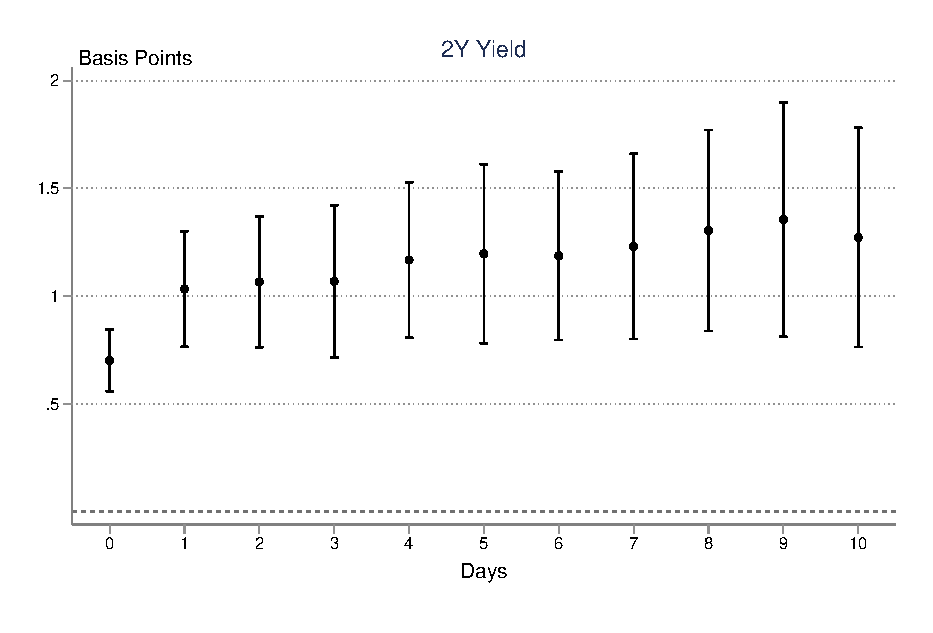
\includegraphics[trim={0.5cm 0cm 0.5cm 0cm},clip,height=.2\textheight,width=1\textwidth]{../Figures/persistprsgmxn02yr.eps} \\
					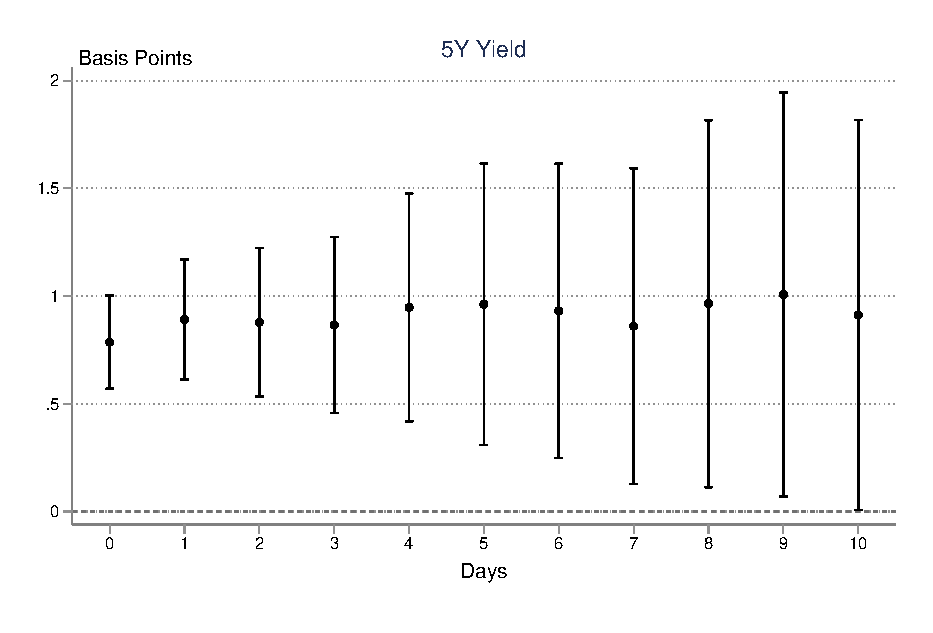
\includegraphics[trim={0.5cm 0cm 0.5cm 0cm},clip,height=.2\textheight,width=1\textwidth]{../Figures/persistprsgmxn05yr.eps} \\
					\includegraphics[trim={0.5cm 0cm 0.5cm 0cm},clip,height=.2\textheight,width=1\textwidth]{../Figures/persistprsgmxn10yr.eps} \\
					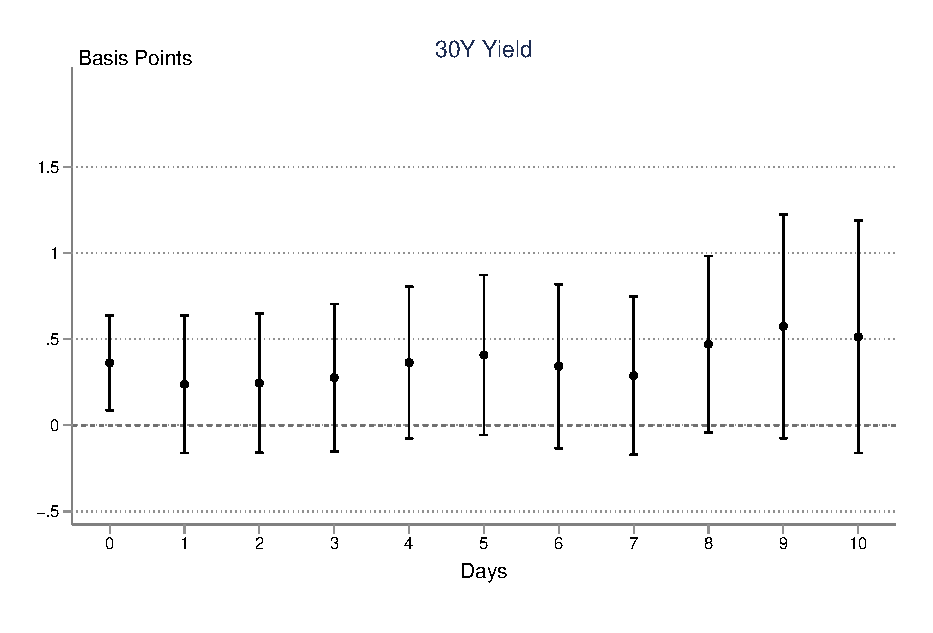
\includegraphics[trim={0.5cm 0cm 0.5cm 0cm},clip,height=.2\textheight,width=1\textwidth]{../Figures/persistprsgmxn30yr.eps} \\
				\end{center}
				\fignotes{This figure plots the coefficient estimates and 95\% confidence intervals for the response of the 2-, 5-, 10- and 30-year yields to policy rate surprises. Yield changes are calculated from close of day \(t - 1\) to day \(t + \idxh\), where \(t\) is a day with a monetary policy announcement and \(\idxh = 0, 1, \ldots, 10\). Announcements are more than ten days apart from each other, see appendix \ref{sec:calendar}. The sample includes all regular monetary policy announcements from January 2011 to \lastobsfx.}
			\end{minipage}
		\end{center}
	\end{figure}
\end{document}
% trim = {<left> <lower> <right> <upper>}

\end{document}

\begin{center}
	[Insert Figure \ref{fig:persistprsyc} here.]
\end{center}

\sectitlespace
\section{DERIVATION OF INCONSISTENCY IN SLOPE ESTIMATOR DUE TO MEASUREMENT ERROR IN DEPENDENT VARIABLE} \label{sec:plim}
\sectitlespace

Let's assume that the variables \(\dpvstar\) and \(\idvstar\) are unobserved, whereas \(\dpv\) and \(\idv\) are observed but measured with an additive error. For ease of exposition, let \(\dpvstar\) and \(\idvstar\) to have zero means. Also, let \(\mean_{i}\), \(\var_{i}\) and \(\covar_{ij}\) denote respectively the expected value and variance of variable \(i\), and the covariance between variables \(i\) and \(j\). 
The model is as follows: 
\begin{equation*} \label{eq:uME}
	\begin{aligned}
		\eqDGP, \\
		\eqMEidv, \\
		\eqMEdpv,
	\end{aligned}
\end{equation*}
\noindent in which the `true' error \(\errortrue\) is i.i.d. with zero mean, variance \(\varE\) and uncorrelated with \(\idvstar\), while the measurement errors \(\merhs\) and \(\melhs\) have zero means, variances \(\varU\) and \(\varV\), and are uncorrelated among themselves and with \(\errortrue\).\footnote{Alternatively, \(\meanE = \meanU = \meanV = \covarEX = \covarUV = \covarUE = \covarVE = 0\).} The estimated equation is thus:
\begin{equation} \label{eq:nDGPme}
	\eqDGPme.
\end{equation}

In the classical measurement error model, the least squares estimators \(\estimB\) and \(\estimSE\) are inconsistent when only the independent variable is measured with error (i.e., \(\varU > 0\), \(\varV = \covarUX = \covarUY = 0\)); the degree of inconsistency depends on an attenuation factor \(\attnfactor\) defined as \(\varXstar /\varX\), so \(0< \attnfactor < 1\).\footnote{ See \textcite{Pischke:2007} for a derivation of \(\eqPlimBstdshort\) and \(\eqPlimSstd\). When there is no measurement error in the independent variable, \(\attnfactor = 1\), in which case \(\estimB\) and \(\estimAVB\) are consistent.} Yet \(\estimB\) is consistent but with a larger standard error when only the dependent variable is measured with error (i.e., \(\varV > 0\), \(\varU = \covarVX = \covarVY = 0\)). 

In validation studies, the measurement errors \(\merhs\) and \(\melhs\) are treated as observed because the `noisy' and `true' values for the dependent and independent variables are observed. This allows me to assess the magnitude of the measurement errors and to test the validity of the classical assumptions. For this purpose, the analysis (as in section \ref{sec:puzzle}) uses the daily and intraday exchange rate returns and policy rate surprises. Table \ref{tab:cevassumptions} reports the values of \(\covar_{\merhs}\) and \(\covar_{\melhs}\), and compares the classical assumptions against the data.\footnote{In addition, the null hypotheses \(\meanU = 0\), \(\meanV = 0\) and \(\corrUV = 0\) are not rejected.} 

%\documentclass[a4paper,10pt]{article}
\usepackage[labelsep=period,labelfont=bf]{caption}
\usepackage{multirow}
\usepackage{tabularx}
\usepackage{booktabs}
\usepackage{threeparttable}
\usepackage{pdflscape}
\input{../Settings/macros_global}			   % Personalized commands
%% Personalized Macros
% Variable Definitions, Equations

%---------------------------------------------------------------
% Variable Definitions
%---------------------------------------------------------------
\providecommand{\tiie}{TIIE28D}
\providecommand{\lastobs}{December 2021}
\providecommand{\lastobsfx}{November 2021}
\providecommand{\lastobsflwbdm}{December 2021}
\providecommand{\lastobsflwtic}{August 2021}
\providecommand{\idxt}{t}
\providecommand{\idxh}{h}
\providecommand{\idxi}{i}
\providecommand{\idxsfwd}{\idxt+\idxh}
\providecommand{\idxslag}{\idxt-1}
\providecommand{\yld}{y}
\providecommand{\ctrls}{z}
\providecommand{\hld}{H}
\providecommand{\depvar}{\Delta \yld_{\idxt}}
\providecommand{\mps}{\Delta x_{\idxt}}
\providecommand{\depvarclean}{\depvar^{*}}
\providecommand{\mpsclean}{\mps^{*}}
\providecommand{\paramB}{\beta}
\providecommand{\intrcpt}{\paramB_{0}}
\providecommand{\slopetrgt}{\paramB_{1}}
\providecommand{\slopepath}{\paramB_{2}}
\providecommand{\assets}{X}
\providecommand{\factors}{F}
\providecommand{\loadings}{\Lambda}
\providecommand{\rotated}{Z}
\providecommand{\rmatrix}{U}
\providecommand{\rtdone}{\rotated_{1}}
\providecommand{\rtdtwo}{\rotated_{2}}
\providecommand{\rtdonereg}{Target_{\idxt}}
\providecommand{\rtdtworeg}{Path_{\idxt}}
\providecommand{\lagidx}{j}
\providecommand{\lagorder}{p}
\providecommand{\lagparam}{\gamma}   %\alpha
\providecommand{\lagoper}{L}
\providecommand{\depvarflw}{\Delta \hld_{\idxt}}
\providecommand{\flows}{w_{\idxt}}
\providecommand{\flowslag}{w_{\idxt - \lagidx}}
\providecommand{\lagsum}{\sum_{\lagidx = 1}^{\lagorder} \lagparam_{\lagidx} \flowslag}
\providecommand{\lagsumh}{\sum_{\lagidx = 1}^{\lagorder} \lagparam^{\lagidx}_\idxh \flowslag}
\providecommand{\dimobs}{T}
\providecommand{\dimassets}{n}
\providecommand{\dimfactors}{k}
\providecommand{\dimnull}{\dimfactors_{0}}
\providecommand{\dimsassets}{\dimobs \times \dimassets}
\providecommand{\dimsfactors}{\dimobs \times \dimfactors}
\providecommand{\dimsloadings}{\dimfactors \times \dimassets}
\providecommand{\errorreg}{\varepsilon_{\idxt}}
\providecommand{\errorfac}{\zeta}
\providecommand{\errorflows}{\nu_{\idxt}}
\providecommand{\Rsqrt}{R^{2}}

\providecommand{\dpv}{y}
\providecommand{\idv}{x}
\providecommand{\omv}{\omega}
\providecommand{\dpvstar}{\dpv^{*}}
\providecommand{\idvstar}{\idv^{*}}
\providecommand{\jobs}{Jobs}
\providecommand{\errortrue}{\varepsilon}
\providecommand{\errormix}{\tau}
\providecommand{\melhs}{\nu}
\providecommand{\merhs}{u}
\providecommand{\mean}{\mu}
\providecommand{\covar}{\sigma}
\providecommand{\corr}{\rho}
\providecommand{\var}{\covar^{2}}
\providecommand{\meanE}{\mean_{\errortrue}}
\providecommand{\meanU}{\mean_{\merhs}}
\providecommand{\meanV}{\mean_{\melhs}}
\providecommand{\varE}{\var_{\errortrue}}
\providecommand{\varU}{\var_{\merhs}}
\providecommand{\varV}{\var_{\melhs}}
\providecommand{\varX}{\var_{\idv}}
\providecommand{\varXstar}{\var_{\idvstar}}
\providecommand{\covarEX}{\covar_{\errortrue \idvstar}}
\providecommand{\covarUE}{\covar_{\merhs \errortrue}}
\providecommand{\covarVE}{\covar_{\melhs \errortrue}}
\providecommand{\covarUX}{\covar_{\merhs \idvstar}}
\providecommand{\covarUY}{\covar_{\merhs \dpvstar}}
\providecommand{\covarVX}{\covar_{\melhs \idvstar}}
\providecommand{\covarVY}{\covar_{\melhs \dpvstar}}
\providecommand{\covarUV}{\covar_{\merhs \melhs}}
\providecommand{\covarWXe}{\covar_{\omv \idv}}
\providecommand{\covarVXe}{\covar_{\melhs \idv}}
\providecommand{\corrUV}{\corr_{\merhs \melhs}}
\providecommand{\corrUX}{\corr_{\merhs \idvstar}}
\providecommand{\corrUY}{\corr_{\merhs \dpvstar}}
\providecommand{\corrVX}{\corr_{\melhs \idvstar}}
\providecommand{\corrVY}{\corr_{\melhs \dpvstar}}
\providecommand{\paramG}{\gamma}
\providecommand{\estimB}{\hat{\paramB}}
\providecommand{\paramSE}{\varE}
\providecommand{\estimSE}{\hat{\paramSE}}
\providecommand{\paramAVB}{s}
\providecommand{\estimAVB}{\hat{\paramAVB}}
\providecommand{\attnfactor}{\lambda}
\providecommand{\plim}{\mathrm{plim}}

\providecommand{\reg}{\delta}
\providecommand{\regVonX}{\reg_{\melhs \idv}}
\providecommand{\regWonX}{\reg_{\omv \idv}}
\providecommand{\regWonXstar}{\reg_{\omv \idvstar}}

%---------------------------------------------------------------
% Equations
%---------------------------------------------------------------
\newcommand{\eqOneFac}{\depvar = \intrcpt + \slopetrgt \mps + \errorreg}
\newcommand{\eqOneFacOV}{\depvar = \intrcpt + \slopetrgt PRS_{\idxt} + \paramB_{2} \Delta VIX_{\idxt} + \paramB_{3} \Delta USY_{\idxt} + \paramB_{4} WTI_{\idxt} + \paramB_{5} \jobs_{\idxt} + \errorreg}
\newcommand{\eqTwoFacP}{\depvar = \intrcpt + \slopetrgt \rtdonereg + \slopepath \rtdtworeg + \errorreg}
\newcommand{\eqTwoFacF}{\depvarflw = \intrcpt + \slopetrgt \rtdonereg + \slopepath \rtdtworeg + \errorreg}
\newcommand{\eqPCA}{\assets = \factors \loadings + \errorfac}
\newcommand{\eqRotation}{\rotated = \factors \, \rmatrix}
\newcommand{\eqFlows}{\flows = \intrcpt + \slopetrgt \rtdonereg + \slopepath \rtdtworeg + \lagsum + \eta^{'} \ctrls_{\idxslag} + \errorflows}
\newcommand{\eqAsym}{\yld_{\idxt} = \intrcpt + \paramB_{1} \rtdonereg \mathds{1} \left(\rtdonereg > 0 \right) + \paramB_{2} \rtdonereg \mathds{1} \left(\rtdonereg < 0 \right) \\ + \paramB_{3} \rtdtworeg \mathds{1} \left(\rtdtworeg > 0 \right) + \paramB_{4} \rtdtworeg \mathds{1} \left(\rtdtworeg < 0 \right) + \errorreg}

\newcommand{\eqDGP}{\dpvstar &= \paramB \idvstar + \errortrue}
\newcommand{\eqDGPme}{\dpv = \paramB \idv + \errormix = \paramB \idv + \eqErrormix}
\newcommand{\eqDGPov}{\dpvstar = \paramB \idvstar + \paramG \omv +  \errortrue}
\newcommand{\eqMEdpv}{\dpv &= \dpvstar + \melhs}
\newcommand{\eqMEidv}{\idv &= \idvstar + \merhs}
\newcommand{\eqAtten}{\attnfactor = \frac{\varXstar}{\varXstar + \varU}}
\newcommand{\eqAttenInLine}{\attnfactor = \varXstar / \left(\varXstar + \varU\right) }
\newcommand{\eqErrormix}{\errortrue - \paramB \merhs + \melhs}

\newcommand{\eqPlimBstd}{\plim \left( \estimB \right) = \frac{cov(\idv, \dpvstar)}{var(\idv)} = \frac{cov(\idvstar + \merhs, \paramB \idvstar + \errortrue)}{var(\idvstar + \merhs)} = \paramB \frac{\varXstar}{\varXstar + \varU} = \paramB \attnfactor}
\newcommand{\eqPlimBstdshort}{\plim (\estimB) = \paramB \attnfactor}

\newcommand{\eqPlimSstd}{\plim \left( \estimAVB \right) = \attnfactor \paramAVB + \attnfactor(1 - \attnfactor) \paramB^{2}}

\newcommand{\eqPlimBnew}{\plim \left( \estimB \right) 
	= \frac{cov(\idv, \dpv)}{var(\idv)} 
	= \frac{cov(\idvstar + \merhs, \paramB \idvstar + \paramG \omv + \errortrue)}{var(\idvstar + \merhs)} 
	= \frac{\paramB \varXstar + \paramG \covarWXe}{\varXstar + \varU}  }

\newcommand{\eqPlimBbias}{\plim \left( \estimB \right)
	= \paramB \frac{\varXstar}{\varX} + \paramG \frac{\covarWXe}{\varX}
	= \paramB \attnfactor + \paramG \regWonX}

\providecommand{\errordepvar}{e_{y}}
\providecommand{\errormps}{e_{x}}
\newcommand{\eqMEdepvar}{\depvar &= \depvarclean + \errordepvar}
\newcommand{\eqMEmps}{\mps &= \mpsclean + \errormps}

\newcommand{\eqLPrhs}{\alpha_{\idxh} + \beta^{1}_{\idxh} \; \rtdonereg +  \beta^{2}_{\idxh} \; \rtdtworeg + \eta^{'}_{\idxh} \ctrls_{\idxslag}  + u_{\idxsfwd}}

\newcommand{\eqLPprices}{\yld_{\idxsfwd} - \yld_{\idxslag} = \eqLPrhs} 

\newcommand{\eqLPflows}{\hld_{\idxsfwd} - \hld_{\idxslag} = \eqLPrhs} 

\newcommand{\eqLP}{\yld_{\idxsfwd} - \yld_{\idxslag} = \alpha_{\idxh} + \gamma_{\idxh} \mps + u_{\idxsfwd}} 			    % Personalized commands
%\pagestyle{empty}

\begin{document}
	\newcolumntype{Y}{>{\centering\arraybackslash}X}
%	\begin{landscape}
	\begin{footnotesize}
		\begin{table}[t]
			\centering
			\begin{threeparttable}
				\caption{Assessment of Assumptions in Classical Measurement Error Models}
				\label{tab:cevassumptions}
				\begin{tabularx}{\textwidth}{cYYY}
					\toprule
					Measurement error in & Assumptions & Data & \(p\)-value \\
					\midrule
					\multirow{3}{*}{Dependent variable only} & \(\covar_{\merhs} = 0\) & \(1.86\) &  \\
					& \(\corrVX = 0\) & \(0.16\) & \(0.149\) \\
					& \(\corrVY = 0\) & \(-0.08\) & \(0.444\) \\
					\midrule %\cmidrule(lr){1-4}
					\multirow{3}{*}{Independent variable only} & \(\covar_{\melhs} = 0\) & \(62.18\)  &  \\
					& \(\corrUX = 0\) & \(-0.01\) & \(0.958\) \\
					& \(\corrUY = 0\) & \(0.08\) & \(0.474\) \\
					\midrule
					 & \(0 < \attnfactor < 1\) & \(0.944\) & \\
					\bottomrule
				\end{tabularx}
				\begin{tablenotes}[para,flushleft]
					\footnotesize \textit{Notes:} This table compares the assumptions in classical measurement error models against the data. Measurement errors are calculated as the difference between daily and intraday changes in the variables. \(\covar_{i}\), \(\var_{i}\) and \(\corr_{ij}\) respectively denote the standard deviation and variance of variable \(i\), and the correlation between variables \(i\) and \(j\). Although the assumptions in the models are expressed in terms of covariances, this table reports correlations. 
					The last column tests the null hypothesis of zero correlation. The attenuation factor is calculated according to \(\eqAttenInLine\), where \(\covar_{\idvstar} = 7.64\). 
					The sample includes all regular monetary policy announcements from January 2011 to \lastobsfx.
				\end{tablenotes}
			\end{threeparttable}
		\end{table}
	\end{footnotesize}
%	\end{landscape}
\end{document}

%lambda = s2x*/(s2x* + s2u) = (7.63747^2)/(1.860757^2+7.63747^2) = 0.9439678251
%lambda = s2x*/s2x = 7.63747^2/7.850536^2 = 0.9464559716

%        c1      c2
%r1   1.861       .
%r2   0.157   0.149
%r3  -0.084   0.444
%r4  62.127       .
%r5  -0.006   0.958
%r6   0.078   0.474
%r7   0.944       .
%
%. di lambda2
%.94645609
%
%. 
%. * Summary
%. summ merhs melhsfx mpswc mpswc_ttdm if idx11 & regular
%
%Variable |        Obs        Mean    Std. dev.       Min        Max
%-------------+---------------------------------------------------------
%merhs |         		86   -.0526744    1.860757       -5.5        5.5
%melhsfx |         		86   -5.605278    62.12722  -152.9995   138.9821
%mpswc |         		86   -.3236047     7.63747      -45.8         16
%mpswc_ttdm |       86   -.3762791    7.850536      -45.8       18.5
%
%. pwcorr melhsfx merhs mpswc usdmxn if idx11 & regular, sig
%
%|  melhsfx    merhs    mpswc   usdmxn
%-------------+------------------------------------
%melhsfx |   1.0000 
%|
%|
%merhs |   0.0860   1.0000 
%|   0.4311
%|
%mpswc |   0.1568  -0.0057   1.0000 
%|   0.1494   0.9583
%|
%usdmxn |  -0.0836   0.0782  -0.5027   1.0000 
%|   0.4439   0.4743   0.0000
%|
%
%. 
%. * Correlations (footnotes in appendix D)
%. pwcorr merhs melhsfx mpswc_ttdm if idx11 & regular, sig
%
%|    merhs  melhsfx mpswc_~m
%-------------+---------------------------
%merhs |   1.0000 
%|
%|
%melhsfx |   0.0860   1.0000 
%|   0.4311
%|
%mpswc_ttdm |   0.2315   0.1729   1.0000 
%|   0.0320   0.1114
%|
%
%.         // No correlation between ME's
%.         // ME on RHS correlates w/ RHS variable measured w/ error -> in line 
%> with CEV assumption
%.         // ME on LHS does not correlate w/ RHS variable measured w/ error -> 
%> no endogeneity bias
%. 
%. * H0's not rejected (footnote)
%. *       H0: mean_u = 0 vs. H1: mean_u != 0
%. *       H0: mean_v = 0 vs. H1: mean_v != 0
%. quiet ttest merhs == 0
%
%. di r(p)
%.33589461
%
%. quiet ttest melhsfx == 0
%
%. di r(p)
%.56800417
\begin{center}
	[Insert Table \ref{tab:cevassumptions} here.]
\end{center}

The reason behind the puzzle is noise in daily exchange rate returns. In the data, the hypothesis \(\corrUX = 0\) is not rejected,\footnote{Alternatively, \(\corr_{\merhs \idv} = 0.23\) is statistically different from zero at the 5\% level.} so the estimator \(\estimB\) in equation (\ref{eq:nDGPme}) will be biased and inconsistent as long as the independent variable is measured with error (\(\covar_{\merhs} \neq 0\)). 
However, \(\covar_{\merhs}\) is relatively small (less than 2 basis points), thus the attenuation factor \(\attnfactor\) is close to 1. Comparing the estimated coefficients in the first two columns of table \ref{tab:factorfx} confirms that attenuation bias is indeed relatively small.\footnote{Since \(\attnfactor\) is the same for the exchange rate and bond yields, the attenuation bias is also relatively small when intraday changes in yields are regressed on daily changes in the 3-month swap.} In contrast, measurement error in the dependent variable is quite large (\(\covar_{\melhs}\) is more than 60 basis points).\footnote{For reference, \(\covar_{\melhs}\) for the 10-year yield is 4.48 basis points.} 

Measurement error in the dependent variable can bias the estimator in two cases. First, if the error is systematically related to the independent variable, creating endogeneity bias. In table \ref{tab:cevassumptions}, however, the error in daily exchange rate returns is not systematically related to the policy rate surprises (\(\corrVX = 0\) and \(\corr_{\melhs \idv} = 0\) are not rejected). 

Measurement error in the dependent variable can also cause bias if the error captures the effects of other variables influencing the exchange rate, generating an omitted variable bias. To address this case, the measurement error model is extended as follows:
\[\eqDGPov,\]
\noindent in which \(\omv\) is the omitted variable (i.e. \(\paramG \neq 0\)) and it is assumed to be uncorrelated with \(\errortrue\), \(\merhs\) and \(\melhs\). The estimated model is again that in equation (\ref{eq:nDGPme}), but in which \(\melhs = \paramG \omv\). The degree of inconsistency in \(\estimB\) is then:
\[\eqPlimBnew\]
\begin{equation} \label{eq:nPlimBbias}
	\eqPlimBbias.
\end{equation}

This inconsistency in \(\estimB\) hence depends on the attenuation factor and a term related to the omitted variable, in which \(\regWonX\) is the slope coefficient from regressing \(\omv\) on \(\idv\).\footnote{If there is no measurement error in \(\idv\) (\(\varU = 0\)), \(\omv\) is regressed on \(\idvstar\) instead of \(\idv\).} The probability limit of \(\estimAVB\) also has an additional term related to \(\omv\). Therefore, there will be bias and imprecision in \(\estimB\) whenever measurement error in the dependent variable captures the effects of an omitted variable (\(\melhs = \paramG \omv\)), even without measurement error in the independent variable (\(\attnfactor = 1\)). The last two columns of table \ref{tab:factorfx} align with this result.

Although the second term in equation (\ref{eq:nPlimBbias}) cannot be assessed directly (because \(\omv\) is unobserved), it can be used to characterize the bias. In particular, the sign of the bias depends on the signs of \(\paramG\) and \(\regWonX\). For instance, an upward bias (\(\paramG \regWonX > 0\)) implies either \(\paramG > 0\) and \(\regWonX > 0\), or \(\paramG < 0\) and \(\regWonX < 0\). 

All the potential omitted variables considered in section \ref{sec:omittedvar} contribute for the estimator to be upward bias. For each variable \(\idxi\), table \ref{tab:prsov} reports \(\regWonXstar^{\idxi}\) and \(\regWonX^{\idxi}\)---from regressing the variables on the policy rate surprises---while table \ref{tab:factorov_fx} reports \(\paramG^{\idxi}\). The signs of the coefficients for the corresponding variables in the two tables are the same, thus \(\paramG^{\idxi} \regWonXstar^{\idxi} > 0\) and \(\paramG^{\idxi} \regWonX^{\idxi} > 0\) for all \(\idxi\). Moreover, the correction of the bias in the last two columns of table \ref{tab:factorov_fx} is close to \(\sum_{\idxi} \paramG^{\idxi} \regWonXstar^{\idxi}\) and \(\sum_{\idxi} \paramG^{\idxi} \regWonX^{\idxi}\).
%\input{../Tables/prsov}
\begin{center}
	[Insert Table \ref{tab:prsov} here.]
\end{center}

%---------------------------------------------------------------
% Tables
%---------------------------------------------------------------
\renewcommand{\thetable}{\thesection\arabic{table}}
\section{Supplementary Table} \label{sec:AppTables}

%\documentclass[a4paper,12pt]{article}
\usepackage[labelsep=period,labelfont=bf]{caption}
\usepackage{multirow}
\usepackage{booktabs}
\usepackage{threeparttable}
\usepackage{pdflscape}
\usepackage{tabularx}
\usepackage{afterpage}
\usepackage[margin=1in]{geometry}
\input{../Settings/macros_global}			   % Personalized commands
%% Personalized Macros
% Variable Definitions, Equations

%---------------------------------------------------------------
% Variable Definitions
%---------------------------------------------------------------
\providecommand{\tiie}{TIIE28D}
\providecommand{\lastobs}{December 2021}
\providecommand{\lastobsfx}{November 2021}
\providecommand{\lastobsflwbdm}{December 2021}
\providecommand{\lastobsflwtic}{August 2021}
\providecommand{\idxt}{t}
\providecommand{\idxh}{h}
\providecommand{\idxi}{i}
\providecommand{\idxsfwd}{\idxt+\idxh}
\providecommand{\idxslag}{\idxt-1}
\providecommand{\yld}{y}
\providecommand{\ctrls}{z}
\providecommand{\hld}{H}
\providecommand{\depvar}{\Delta \yld_{\idxt}}
\providecommand{\mps}{\Delta x_{\idxt}}
\providecommand{\depvarclean}{\depvar^{*}}
\providecommand{\mpsclean}{\mps^{*}}
\providecommand{\paramB}{\beta}
\providecommand{\intrcpt}{\paramB_{0}}
\providecommand{\slopetrgt}{\paramB_{1}}
\providecommand{\slopepath}{\paramB_{2}}
\providecommand{\assets}{X}
\providecommand{\factors}{F}
\providecommand{\loadings}{\Lambda}
\providecommand{\rotated}{Z}
\providecommand{\rmatrix}{U}
\providecommand{\rtdone}{\rotated_{1}}
\providecommand{\rtdtwo}{\rotated_{2}}
\providecommand{\rtdonereg}{Target_{\idxt}}
\providecommand{\rtdtworeg}{Path_{\idxt}}
\providecommand{\lagidx}{j}
\providecommand{\lagorder}{p}
\providecommand{\lagparam}{\gamma}   %\alpha
\providecommand{\lagoper}{L}
\providecommand{\depvarflw}{\Delta \hld_{\idxt}}
\providecommand{\flows}{w_{\idxt}}
\providecommand{\flowslag}{w_{\idxt - \lagidx}}
\providecommand{\lagsum}{\sum_{\lagidx = 1}^{\lagorder} \lagparam_{\lagidx} \flowslag}
\providecommand{\lagsumh}{\sum_{\lagidx = 1}^{\lagorder} \lagparam^{\lagidx}_\idxh \flowslag}
\providecommand{\dimobs}{T}
\providecommand{\dimassets}{n}
\providecommand{\dimfactors}{k}
\providecommand{\dimnull}{\dimfactors_{0}}
\providecommand{\dimsassets}{\dimobs \times \dimassets}
\providecommand{\dimsfactors}{\dimobs \times \dimfactors}
\providecommand{\dimsloadings}{\dimfactors \times \dimassets}
\providecommand{\errorreg}{\varepsilon_{\idxt}}
\providecommand{\errorfac}{\zeta}
\providecommand{\errorflows}{\nu_{\idxt}}
\providecommand{\Rsqrt}{R^{2}}

\providecommand{\dpv}{y}
\providecommand{\idv}{x}
\providecommand{\omv}{\omega}
\providecommand{\dpvstar}{\dpv^{*}}
\providecommand{\idvstar}{\idv^{*}}
\providecommand{\jobs}{Jobs}
\providecommand{\errortrue}{\varepsilon}
\providecommand{\errormix}{\tau}
\providecommand{\melhs}{\nu}
\providecommand{\merhs}{u}
\providecommand{\mean}{\mu}
\providecommand{\covar}{\sigma}
\providecommand{\corr}{\rho}
\providecommand{\var}{\covar^{2}}
\providecommand{\meanE}{\mean_{\errortrue}}
\providecommand{\meanU}{\mean_{\merhs}}
\providecommand{\meanV}{\mean_{\melhs}}
\providecommand{\varE}{\var_{\errortrue}}
\providecommand{\varU}{\var_{\merhs}}
\providecommand{\varV}{\var_{\melhs}}
\providecommand{\varX}{\var_{\idv}}
\providecommand{\varXstar}{\var_{\idvstar}}
\providecommand{\covarEX}{\covar_{\errortrue \idvstar}}
\providecommand{\covarUE}{\covar_{\merhs \errortrue}}
\providecommand{\covarVE}{\covar_{\melhs \errortrue}}
\providecommand{\covarUX}{\covar_{\merhs \idvstar}}
\providecommand{\covarUY}{\covar_{\merhs \dpvstar}}
\providecommand{\covarVX}{\covar_{\melhs \idvstar}}
\providecommand{\covarVY}{\covar_{\melhs \dpvstar}}
\providecommand{\covarUV}{\covar_{\merhs \melhs}}
\providecommand{\covarWXe}{\covar_{\omv \idv}}
\providecommand{\covarVXe}{\covar_{\melhs \idv}}
\providecommand{\corrUV}{\corr_{\merhs \melhs}}
\providecommand{\corrUX}{\corr_{\merhs \idvstar}}
\providecommand{\corrUY}{\corr_{\merhs \dpvstar}}
\providecommand{\corrVX}{\corr_{\melhs \idvstar}}
\providecommand{\corrVY}{\corr_{\melhs \dpvstar}}
\providecommand{\paramG}{\gamma}
\providecommand{\estimB}{\hat{\paramB}}
\providecommand{\paramSE}{\varE}
\providecommand{\estimSE}{\hat{\paramSE}}
\providecommand{\paramAVB}{s}
\providecommand{\estimAVB}{\hat{\paramAVB}}
\providecommand{\attnfactor}{\lambda}
\providecommand{\plim}{\mathrm{plim}}

\providecommand{\reg}{\delta}
\providecommand{\regVonX}{\reg_{\melhs \idv}}
\providecommand{\regWonX}{\reg_{\omv \idv}}
\providecommand{\regWonXstar}{\reg_{\omv \idvstar}}

%---------------------------------------------------------------
% Equations
%---------------------------------------------------------------
\newcommand{\eqOneFac}{\depvar = \intrcpt + \slopetrgt \mps + \errorreg}
\newcommand{\eqOneFacOV}{\depvar = \intrcpt + \slopetrgt PRS_{\idxt} + \paramB_{2} \Delta VIX_{\idxt} + \paramB_{3} \Delta USY_{\idxt} + \paramB_{4} WTI_{\idxt} + \paramB_{5} \jobs_{\idxt} + \errorreg}
\newcommand{\eqTwoFacP}{\depvar = \intrcpt + \slopetrgt \rtdonereg + \slopepath \rtdtworeg + \errorreg}
\newcommand{\eqTwoFacF}{\depvarflw = \intrcpt + \slopetrgt \rtdonereg + \slopepath \rtdtworeg + \errorreg}
\newcommand{\eqPCA}{\assets = \factors \loadings + \errorfac}
\newcommand{\eqRotation}{\rotated = \factors \, \rmatrix}
\newcommand{\eqFlows}{\flows = \intrcpt + \slopetrgt \rtdonereg + \slopepath \rtdtworeg + \lagsum + \eta^{'} \ctrls_{\idxslag} + \errorflows}
\newcommand{\eqAsym}{\yld_{\idxt} = \intrcpt + \paramB_{1} \rtdonereg \mathds{1} \left(\rtdonereg > 0 \right) + \paramB_{2} \rtdonereg \mathds{1} \left(\rtdonereg < 0 \right) \\ + \paramB_{3} \rtdtworeg \mathds{1} \left(\rtdtworeg > 0 \right) + \paramB_{4} \rtdtworeg \mathds{1} \left(\rtdtworeg < 0 \right) + \errorreg}

\newcommand{\eqDGP}{\dpvstar &= \paramB \idvstar + \errortrue}
\newcommand{\eqDGPme}{\dpv = \paramB \idv + \errormix = \paramB \idv + \eqErrormix}
\newcommand{\eqDGPov}{\dpvstar = \paramB \idvstar + \paramG \omv +  \errortrue}
\newcommand{\eqMEdpv}{\dpv &= \dpvstar + \melhs}
\newcommand{\eqMEidv}{\idv &= \idvstar + \merhs}
\newcommand{\eqAtten}{\attnfactor = \frac{\varXstar}{\varXstar + \varU}}
\newcommand{\eqAttenInLine}{\attnfactor = \varXstar / \left(\varXstar + \varU\right) }
\newcommand{\eqErrormix}{\errortrue - \paramB \merhs + \melhs}

\newcommand{\eqPlimBstd}{\plim \left( \estimB \right) = \frac{cov(\idv, \dpvstar)}{var(\idv)} = \frac{cov(\idvstar + \merhs, \paramB \idvstar + \errortrue)}{var(\idvstar + \merhs)} = \paramB \frac{\varXstar}{\varXstar + \varU} = \paramB \attnfactor}
\newcommand{\eqPlimBstdshort}{\plim (\estimB) = \paramB \attnfactor}

\newcommand{\eqPlimSstd}{\plim \left( \estimAVB \right) = \attnfactor \paramAVB + \attnfactor(1 - \attnfactor) \paramB^{2}}

\newcommand{\eqPlimBnew}{\plim \left( \estimB \right) 
	= \frac{cov(\idv, \dpv)}{var(\idv)} 
	= \frac{cov(\idvstar + \merhs, \paramB \idvstar + \paramG \omv + \errortrue)}{var(\idvstar + \merhs)} 
	= \frac{\paramB \varXstar + \paramG \covarWXe}{\varXstar + \varU}  }

\newcommand{\eqPlimBbias}{\plim \left( \estimB \right)
	= \paramB \frac{\varXstar}{\varX} + \paramG \frac{\covarWXe}{\varX}
	= \paramB \attnfactor + \paramG \regWonX}

\providecommand{\errordepvar}{e_{y}}
\providecommand{\errormps}{e_{x}}
\newcommand{\eqMEdepvar}{\depvar &= \depvarclean + \errordepvar}
\newcommand{\eqMEmps}{\mps &= \mpsclean + \errormps}

\newcommand{\eqLPrhs}{\alpha_{\idxh} + \beta^{1}_{\idxh} \; \rtdonereg +  \beta^{2}_{\idxh} \; \rtdtworeg + \eta^{'}_{\idxh} \ctrls_{\idxslag}  + u_{\idxsfwd}}

\newcommand{\eqLPprices}{\yld_{\idxsfwd} - \yld_{\idxslag} = \eqLPrhs} 

\newcommand{\eqLPflows}{\hld_{\idxsfwd} - \hld_{\idxslag} = \eqLPrhs} 

\newcommand{\eqLP}{\yld_{\idxsfwd} - \yld_{\idxslag} = \alpha_{\idxh} + \gamma_{\idxh} \mps + u_{\idxsfwd}} 			    % Personalized commands
%\pagestyle{empty}

\begin{document}
%	\afterpage{
		\begin{normalsize}
			%			\begin{landscape}
			\begin{table}[tbh]
				\begin{center}
					\caption{10-Year Yield Response to Policy Rate Surprises and Omitted Variables} \label{tab:factorov_10y} %: Intraday Data
					\begin{threeparttable}
						\estauto{../Tables/f_factorov_10y.tex}{4}
						\tabnote{This table shows the coefficient estimates in regressions of daily changes in the 10-year yield on \textchange{policy rate surprises (PRS)}, controlling for potential omitted variables. \textchange{The surprises are calculated using both intraday and daily data.} The control variables are the daily change in the VIX, the daily change in the 2-year U.S. Treasury yield, the WTI crude oil price and the surprise in releases of U.S. initial jobless claims (\(IJC \, surprise\)). Daily changes are calculated around monetary policy announcements; intraday changes are calculated from 10 minutes before to 20 minutes after an announcement. The sample includes all regular monetary policy announcements from January 2011 to \lastobsfx. Figures are expressed in basis points. No constant is included in the regressions. \textchange{Heteroskedasticity-robust} standard errors are shown in parentheses. *, **, *** asterisks respectively indicate significance at the 10\%, 5\% and 1\% level.}
					\end{threeparttable}
				\end{center}
			\end{table}
			%			\end{landscape}
		\end{normalsize}
%	}
\end{document}
\begin{center}
	[Insert Table \ref{tab:factorov_10y} here.]
\end{center}

\newpage

\begin{landscape}
	\newpage
\end{landscape}